% Activate the following line by filling in the right side. If for example the name of the root file is Main.tex, write
% "...root = Main.tex" if the chapter file is in the same directory, and "...root = ../Main.tex" if the chapter is in a subdirectory.
 
%!TEX root =  ../Thesis.tex

\chapter[Background Estimation]{Background Estimation}

Once the background has been reduced as much as practical using the trigger and kinematic cuts,
a reliable estimate of the shape and size of the remaining background is critical to optimizing
the exclusion limits.  As detailed in Section~\ref{sec:mass_res}, since the reconstructed mass peak 
of the leading two $b$-jets is so
broad in signal, a mis-estimation of the background shape can lead to systematic errors that
could wash out any possible signal (or worse, be mistaken for a signal where there is none).  

At the same time, the backgrounds in this analysis are challenging to estimate, either in Monte
Carlo simulations or using data-driven methods.  Therefore, much of the work of this analysis is dedicated
to validating the background, especially its shape in jet $p_T$, $m_{bb}$, and so on.
of the background.  

\section{Background Estimation Strategy}
\label{sec:background_strategy}
As QCD is the dominant background in this analysis, it is important to understand
what flavors of QCD jets compose the population of events that survive the cut
chain.  In order to do this, we apply the trigger and cut chain detailed in Chapter~\ref{chap:trig_cuts}.

Once the events have been passed through the cut chain, 
the signal and background are split into 3 exclusive regions based on the $b$-tag weight of the
third jet in the event\footnote{as noted below, the ``third jet'' moniker does not strictly
mean the third-highest $p_T$ jet in the event; rather, it is the jet with the highest $b$-tag weight
that is \textit{not} one of the leading two jets in $p_T$, which are already $b$-tagged coming
out of the cut chain}:
\begin{itemize}
    \item \textit{bbb}: one or more jets (in addition to the two triple-tagged jets) passing a tight (60\% $b$-jet efficiency working point)
 MV1\footnote{recall that MV1 is the name of the offline $b$-tagging algorithm used in most ATLAS analyses} cut
    \item \textit{bbloose}: events failing the \textit{bbb} classification but which have one or more jets passing a loose (80\% efficiency
 working point) MV1 cut
    \item \textit{bbanti}: events that have no jets passing an 80\% MV1 cut-–effectively a veto on the presence of any
 $b$-tagged jets other than those firing the trigger
\end{itemize}

When assigning events to one of these categories, we only allow $b$-tags on the leading
five jets to count toward the $bbb$ or $bbloose$ categories.  In other words, if the third
$b$-tagged jet in an event is the 6th jet (in $p_T$ ordering) overall, the event 
will be classified as $bbanti$.  This requirement is motivated by our physics awareness that
the $b$-jets coming from signal events should be fairly high $p_T$, so this should have
a minimal effect of rejecting signal that would otherwise be accepted.  On the other
hand, with high-jet-multiplicity QCD events, there is the combinatorial effect of looking across
more jets for $b$-tags that increases the likelihood of an event being classified as signal-like
(\textit{bbb} or \textit{bbloose}) as there are more jets in the event.  Only looking at the leading 5 jets
for $b$-tags keeps this effect under control. 

Once all the events have been categorized, the search proceeds by fitting the background
in the \textit{bbanti} region, which we sometimes refer to as the \textit{bbanti}
control region.  The events in this category will be mostly QCD background, especially
$b\bar{b}$ QCD, although about 20\% of the signal might fall into this category.  The 
\textit{bbb} category will be enriched in $b\bar{b}b$ events, either from signal
or QCD background, although 60\% of the signal falls into this category and the QCD 
backgrounds are much lower when a third $b$-jet is required.  The background estimation
strategy for this analysis is to fit the $m_{bb}$ distribution in the background-dominated
\textit{bbanti} category, and use that shape to predict the background shape in the \textit{bbb}
signal region.   The extrapolation from \textit{bbanti} to \textit{bbb} is validated using the 
bb QCD MC sample described in Section~\ref{sec:bb_qcd_mc}.

\section{Background Estimation Method Based on Parameterized Histogram Fitting}
The background consists almost exclusively of QCD with 2 or more real $b$-jets, which 
fortunately has a $m^{'}_{bb}$\footnote{the $m^{'}_{bb}$ variable is described in more detail
immediately below, and in Section~\ref{sec:rotation}} spectrum that does not have any peaks or other difficult
structure above about 350 GeV.  Below that mass, the trigger turn-on curve becomes
a major feature of the spectrum.  Above that mass, there
is a smoothly falling distribution that we fit to an RhhBinnedPdf, which is a parameterized
histogram PDF that is also used for fitting the signal.

In a few words, the background fit strategy proceeds in the following way:
\begin{itemize}
    \item Start with a signal mass point
    \item Apply a mass-point-specific rotation based on the the eigenvectors of 
    the signal MC sample of that mass point, as calculated using $m_{bb}$, $p_{T,1}$ and $p_{T,2}$; we call 
    the components of this rotated basis $m_{bb}'$, $p_T^{1'}$ and $p_T^{2'}$ (more
    details in Section~\ref{sec:rotation}).  Briefly, the $m^{'}_{bb}$ variable
    is a linear combination of $m_{bb}$, $p_{T,1}$ and $p_{T,2}$, which has a shape
    similar to $m_{bb}$ but exploits correlations in the signal to suppress the backgrounds.
    \item Apply cuts to $p^{'}_{T,1}$ and $p^{'}_{T,2}$, and use $m_{bb}^{'}$ as the final 
    discriminating variable 
    \item Fit the $m_{bb}^{'}$ distributions within the range -50 GeV $<m_{bb}^{'}<$350
    with a parameterized histogram, separately for each $b$-tag and $n_{jets}$ category
    in signal MC.
    \item Fit the data in the same $m_{bb}^{'}$ range, also with a parameterized histogram,
    but fit all tag categories together.  In other words, all 3-jet events (whether in the
    $bbb$, $bbloose$, or $bbanti$ tag category) are fit with the same histogram in data.
    This has the practical effect of $bbanti$ dominating the fit result because of its
    higher statistics, so the resulting
    histogram is dominated by the $m_{bb}^{'}$ distribution in background tag categories.
    \item Fix the signal shape to the fits found in MC
    \item Create a composite PDF that is the sum of the background and signal components
    \item Initialize the parameters of the background component to the final parameter values
    found in the background-only fit, but allow the background parameters to float in 
    the fitting procedure
    \item Fit the data in the signal region, allowing the background shape, background
    normalization, and signal normalization to float
    \item Repeat for the next signal mass point
\end{itemize}

Although we have signal MC with $m_A$ values as low as 250 GeV, this fit strategy only
begins to work above $m_A=$400 GeV, because of the trigger turn-on curve.  The signal mass 
points to which we would have sensitivity range from 400 to 800 GeV (potentially higher,
but 800 GeV is our highest signal MC point). 

While the analysis was in development, it was blinded to avoid bias.  This was done 
by removing \textit{bbb} events from the data, and replacing them with a sample of
events with the same normalization drawn from the \textit{bbanti} distribution
in data.  For the final search, the \textit{bbb} events were substituted back in.



%\section{Turn-On Curve Modeling}
%Although the lowest part of the $m_{bb}$ distribution (below 300 GeV) is not part of the search regime,
%because of the rapidly changing background, including it in the background model helps
%improve the overall fit by allowing for a slightly fewer events at moderately low
%$m_{bb}$ (between about 300 and 400 GeV) than an exponential alone would predict.
%The turn-on is fit with a logistic function of the form

%\begin{equation}
%f(m_{bb}) = N\frac{1}{1+e^{-c(m_{bb}+d)}}
%\end{equation}

%In this equation, N controls the overall normalization, $c$ governs the steepness
%of the turn-on curve, and $d$ is the horizontal offset.

%\textbf{once we confirm this (or something like it) as the final fit model,
%add a plot showing how this function changes with c/d and the composite
%model of exponential times logistic}


\section{Modeling of Background Shape}
\subsection{Selection of Parameterized Histogram}
Once the rotation and cuts have been applied, the data is fed into an 
binned maximum likelihood fit for mathematical modeling.  The fitting
of both signal and background is done in RooFit.  There are a number 
of candidate models for the background fit, which can be evaluated
both on their goodness-of-fit (as measured by a metric like $\chi^2/DOF$)
and their ease of convergence.

A number of mathematical functions were attempted in fitting the
background, but in the final analysis, a parameterized histogram was
used in part because of its easier convergence on background, and
in part it allowed us to avoid an unstable functional fit to the signal.

The important compromise of fitting to a histogram for the
background is that it removes some of the constraints that a functional
fit provides (for example, a decaying exponential imposes the constraint
that the background is always decreasing as $m^{'}_{bb}$ increases, 
but a histogram could fluctuate up in the case of an excess).  That 
means that we must rely on our background-dominated $bbanti$ region
to understand the shape of the background, and then extrapolate that
shape to the $bbb$ signal region in order to look for deviations from
the background-only hypothesis.  The extrapolation must be validated in 
background MC: the assumption this method makes is that the $m^{'}_{bb}$
distribution is the same regardless of the flavor of the third jet 
in the event.  If that assumption holds, this extrapolation method is a
valid way to predict the background shape in the signal region.


The probability density functions (PDFs) for $m^{'}_{bb}$ are based on a parameterized step function,
which is equivalent to parameterizing a normalized histogram in terms of the content of each
bin. The number of needed parameters correspond to the number of bins minus one
(because of the normalization). Using directly the bin content in each bin
$b_{i}$ would induce an unstable behavior, since the last bin
content would need to be parameterized as $1-\sum_{i=1}{(N_{bins}-1)} b_{i}$
and the fit would easily converge to configurations where the last bin is negative,
and at that point convergence is spoiled. Instead, the values of $p_{i}$
are re-parameterized in terms of another set of parameters
$b_{i}$\footnote{This nice trick was introduced for the first time by Aaron Roodman (SLAC) in the BaBar experiment}.

\begin{itemize}
\item $b_{1} = p_{1}$
\item $b_{2} = p_{2} \left(1-p_{1}\right)$
\item $b_{3} = p_{3} \left(1-p_{2} \right) \left( 1-p_{3}) \right)$
\item $....$
\end{itemize}
With this choice all parameters $p_{i}$ with $i$ from 
1 to $N-1$ can be limited to $[0,1]$, without loss of generality, 
and the fit will always converge reliably, provided the dataset the fit is applied 
to has at least one event in each bin of the PDF.

In the final fit to the data sample the following parameters are extracted:
\begin{itemize}
\item The signal strength $\mu$;
\item The background normalizations $N_{bkg,l}$, separately in each category;
\item The  background $PDF_{bkg}(m_{bb})$, which is allowed to vary across categories (both in shape and normalization).
\end{itemize} 


Although the final fit model was a histogram, the following functions were
also considered and we discuss below the behavior they exhibited:
%In brief, the functions given consideration include the following:
\begin{itemize}
    \item Bernstein Polynomial
    \item Power Decay Series
    \item Decaying Exponential with 1 parameter
    \item Decaying Exponential with 2 parameters
\end{itemize}

\subsubsection{Bernstein Polynomials}
The Bernstein polynomials are a family of polynomials that are characterized
particularly by their attractive feature of being positive-definite, or never
predicting a negative value for a PDF composed of them.  However, we find
that it takes a high degree of polynomial (5 parameters or more) to fit the
background over the full mass range, and a polynomial with a 
degree this high struggles (and often fails) to converge.  Moreover, a
drawback of high-degree polynomials is their capability to ``wiggle'' and
potentially absorb a signal within the background model.

\subsubsection{Power Decay Series}
A power decay series of the form $\frac{a}{x} + \frac{b}{x^3} + \frac{c}{x^5} + ...$
is another possibility; if all the powers of $x$ in the denominators are
odd, this series cannot wiggle like the Bernstein polynomials.  However,
a simple series with a few terms does not fit the background shape well 
over the full mass range, and when many terms are added to the series then
the fit struggles to find a global maximum of the likelihood function, leading
to non-convergence.

\subsubsection{Decaying Exponential with 1 Parameter}
Like a decaying power series, a decaying exponential function is monotonically
decreasing; however, unlike a power series, an exponential with a single
parameter (i.e. a model of the form $f(x)=e^{-x/\tau}$) provides 
a relatively good fit to the background distribution in most tag and jet
categories, with $\chi^2/DOF$ values below 2 for all \textit{bbb} and \textit{bbloose}
distributions \footnote{the \textit{bbanti} distributions prove harder to
fit with a 1-parameter exponential, with $\chi^2/DOF$ values between 2.8 and 3.9}.
Additionally, the simplicity of a 1-parameter exponential means that the
fits converge quickly and reliably over the full mass range.

\subsubsection{Decaying Exponential with 2 Parameters}
A decaying exponential with two parameters (i.e. a model of the form  $f(x)=e^{-x/\tau+\omega x^2}$)
has some of the same nice features of a single-parameter exponential (simple functional
form, no possibility of signal-spoofing wiggles) while offering
more flexibility than the 1-parameter exponential.  The $\chi^2/DOF$ and pulls
for the 2-parameter exponential fits reflect this flexibility to better
fit the data, every jet/tag category has a fit that is as good or better
for the 2-parameter exponential as for the 1-parameter exponential.  In 
particular, the \textit{bbanti} categories that have higher $\chi^2/DOF$ values
in the 1-parameter fit show $\chi^2/DOF$ results of 1.0-1.2 with the 2-parameter fits. 
However, the convergence of this model (especially when it is used in a composite
model that can also include signal) can be tricky, and we found that in practice
the parameters need to be initialized and constrained very precisely to get
good results.  We also found that this model was prone to introducing spurious
signal when used in combination with our signal, so that even when running in 
configurations where no signal was present, the fit was prone to returning
a nonzero signal cross section.


%%% START HERE


\subsection{Validation of Background Shape Extrapolation}
A critical assumption of this fit method is that the shape of the $m_{bb}$ distribution
in background does not vary based on the flavor (or, relatedly, $b$-tag status)
of the third jet in the event.  We validate this assumption in the $b$-jet enriched 
QCD MC sample detailed in Section~\ref{sec:bb_qcd_mc}

As detailed in Section~\ref{sec:rotation}, our final discriminating variable is actually
not $m_{bb}$ but a variable we call $m_{bb}^{'}$, 
which is a linear combination of $m_{bb}$, $p_{T,1}$ and $p_{T,2}$.  So while we
do check that the $m_{bb}$ distributions are not biased by the flavor of the third jet,
the real figure of merit lies in showing that $m_{bb}^{'}$ is not biased by the
flavor of the third jet either.  The plots in Figure~\ref{fig:bkg_shape_compare}
show $m_{bb}^{'}$ in the $bbb$ and $bbanti$ tag categories, with a ratio plot drawn below
to see any shape differences more clearly.  Although not all the bins agree 
exactly between the \textit{bbb} and \textit{bbanti} categories, there is little sign of a bias in the 3-jet
or 4-jet categories; the 5-jet category shows a slight shape difference at high values
of $m_{bb}^{'}$ for which we assign a systematic error (more details in Section~\ref{sec:background_syst}).

\begin{figure}[hbt]
\includegraphics[width=0.45\linewidth]{BackgroundEstimation/mbb_bbb_3jets_rotated.eps}
\includegraphics[width=0.45\linewidth]{BackgroundEstimation/mbb_bbb_4jets_rotated.eps}
\includegraphics[width=0.45\linewidth]{BackgroundEstimation/mbb_bbb_5jets_rotated.eps}
\caption{The distributions of the final discriminating variable, $m_{bb}^{'}$, 
in background MC for the $bbanti$ and $bbb$ tag categories.  The three different plots
compare the 3-jet, 4-jet, and 5-or-more jet categories.  No signs of major shape
differences are seen.
\label{fig:bkg_shape_compare}}
\end{figure}




 


%Following the prescription in the Standard Model $h\rightarrow\gamma\gamma$
%search \cite{spurious_signal}, the model must meet at least one of the following
%criteria:

%\begin{itemize}
%    \item $N_{sp}<$ 10\% $N_{s,exp}$
%    \item $N_{sp}<$ 20\% $\sigma_{bkg}$
%\end{itemize}

%$N_{s,exp}$ is the number of signal events expected to pass the event selection cuts, and 
%$\sigma_{bkg}$ is the statistical uncertainty on the number of background events when
%fitting the signal+background model to the background-only Asimov dataset.

%\textbf{fill in results of these tests after they have been completed}


\subsection{Non-QCD Background}
\label{sec:non_qcd_bkgs}

\subsubsection{All-Hadronic $t\bar{t}$ Background}
When $t\bar{t}$ decays all-hadronically, it can create events with several high-$p_T$
jets and two or more $b$-tagged jets (where the $b$-tags come from both real $b$-quarks
and from mistagged light flavor).  We anticipate that, because it has a production
cross section that is much smaller than QCD\footnote{this statement depends somewhat
on cuts, $b$-tagging, etc., but as explained below it does turn out to be the case
in the relevant region in phase space for this analysis}, $t\bar{t}$ will not be a major background.
We confirm this assumption in MC by using the all-hadronic $t\bar{t}$ sample summarized
in Table~\ref{tab:ttbar_params}.


We find that in Pythia MC simulations, all-hadronic $t\bar{t}$ has an efficiency of 7.5\% after
the EF\_2j35\_loose\_j145\_j35\_a4tchad trigger, and approximately 2\% efficiency
in the offline cuts relative to the trigger.  Estimating the $t\bar{t}$ cross section
as 165 pb, and a 44\% branching ratio in the all-hadronic decay channel, this gives
a 0.11 pb $t\bar{t}$ cross section expected after the trigger and offline cuts.  In the
full 2012 dataset, this amounts to about 2400 events.  While
this is not a negligible cross section compared to the signal, it is more than an
order of magnitude smaller than the QCD background.

In addition to checking the magnitude of the $t\bar{t}$ background, we check the shape
for any shape differences in the $m_{bb}$ distribution depending on the tag status of the
third jet, and do not find any major discrepancies that point toward $t\bar{t}$ as a
potential peaking background in the signal region. The $m_{bb}$ distributions in the
bbb, bbloose and bbanti bins for the all-hadronic $t\bar{t}$ can be found in Figure
~\ref{fig:ttbar_mbb}.




\begin{figure}[hbt]
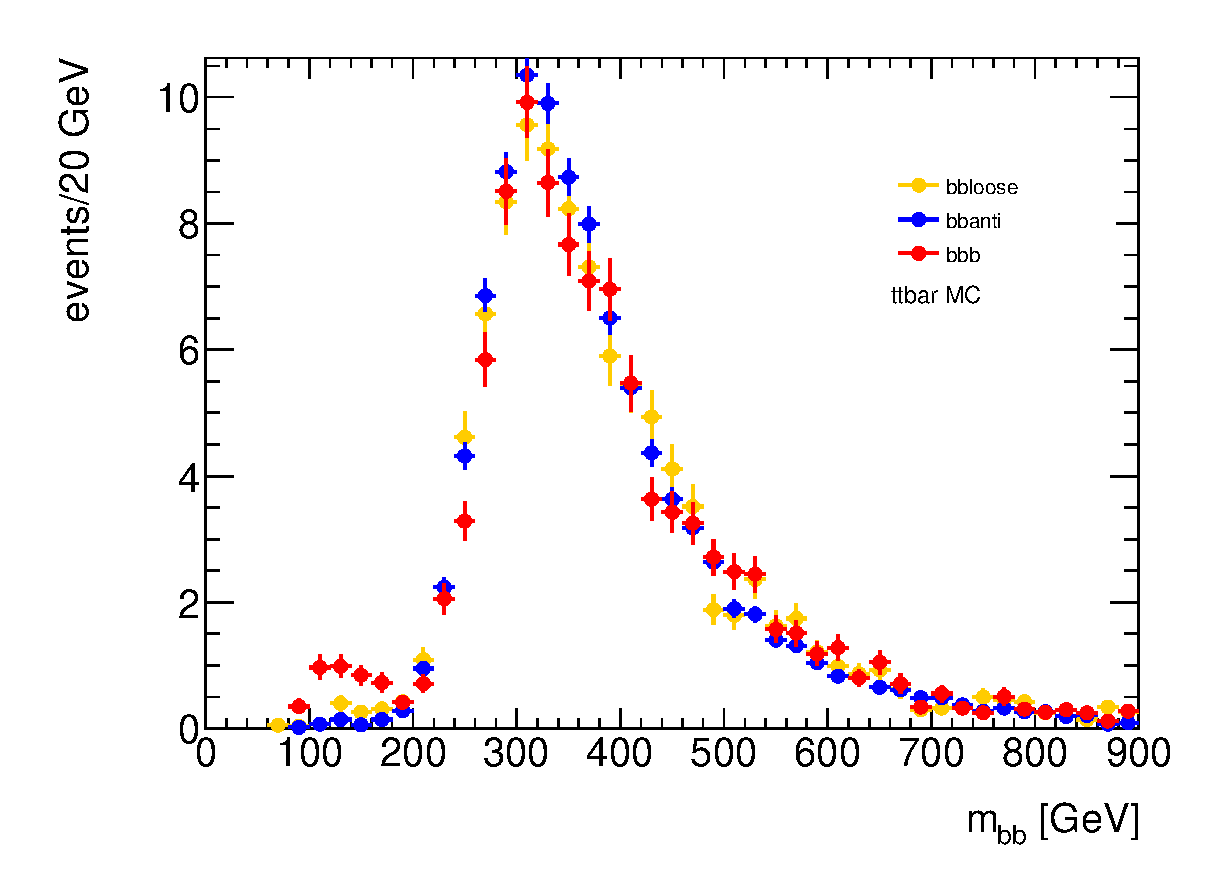
\includegraphics[width=0.45\linewidth]{BackgroundEstimation/images/mbb_compare_bbb_bbloose_bbanti_ttbar.eps}
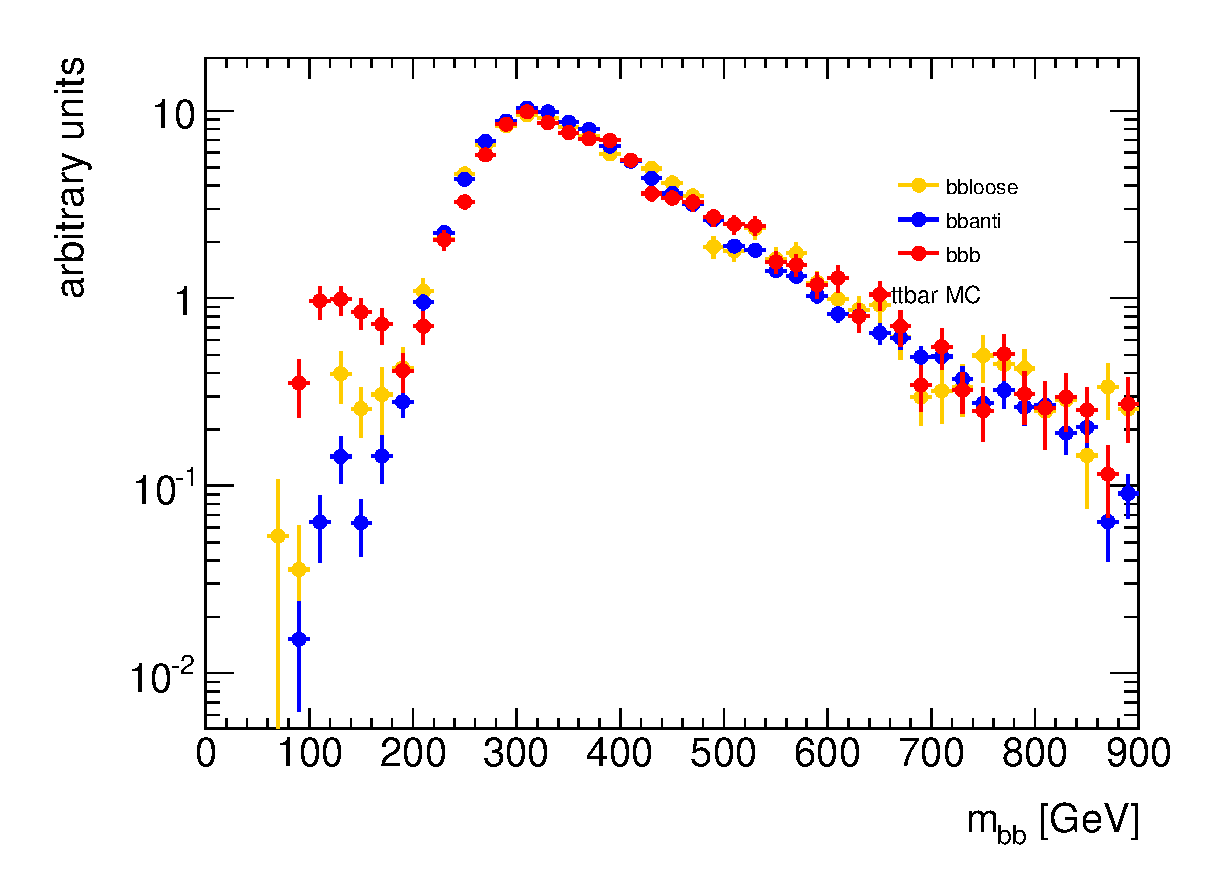
\includegraphics[width=0.45\linewidth]{BackgroundEstimation/images/mbb_compare_bbb_bbloose_bbanti_ttbar_logy.eps}
\caption{The $m_{bb}$ distributions for all-hadronic $t\bar{t}$ MC after the trigger and all offline cuts are applied (linear Y axis on the left, logarithmic scale on the right).  In addition to the overall cross-section, we also want to probe any shape differences that arise when the tag status changes on the third jet in the event.  No significant shape differences are seen.}
\label{fig:ttbar_mbb}
\end{figure}

















